


\tikzset{every picture/.style={line width=0.75pt}} %set default line width to 0.75pt        

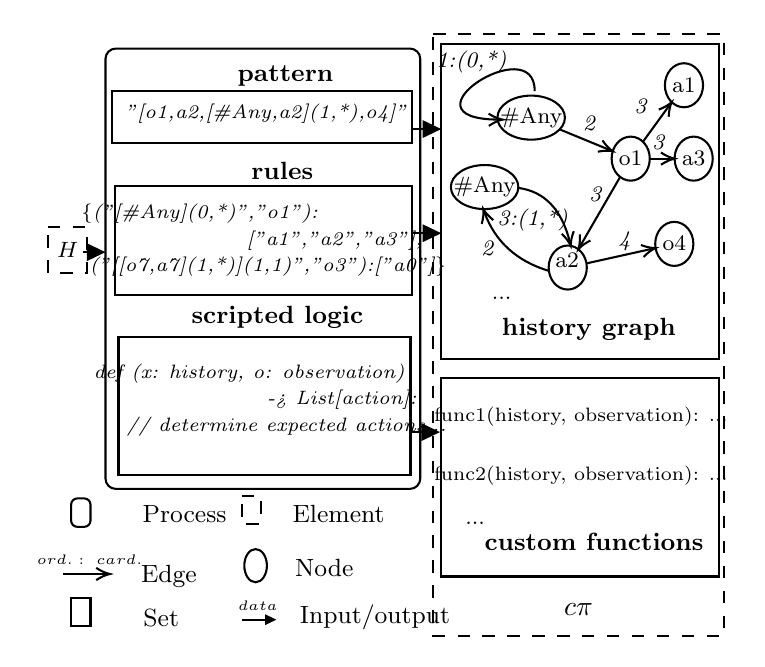
\begin{tikzpicture}[x=0.75pt,y=0.75pt,yscale=-1,xscale=1]
%uncomment if require: \path (0,2639); %set diagram left start at 0, and has height of 2639

%Shape: Rectangle [id:dp054521411752182836] 
\draw   (259.89,1693.39) -- (393.67,1693.39) -- (393.67,1789.2) -- (259.89,1789.2) -- cycle ;
%Curve Lines [id:da8374141983399681] 
\draw    (304.89,1555.38) .. controls (305.21,1525.3) and (237.19,1569) .. (287.76,1569.07) ;
\draw [shift={(289.33,1569.06)}, rotate = 179.11] [color={rgb, 255:red, 0; green, 0; blue, 0 }  ][line width=0.75]    (6.56,-2.94) .. controls (4.17,-1.38) and (1.99,-0.4) .. (0,0) .. controls (1.99,0.4) and (4.17,1.38) .. (6.56,2.94)   ;
%Shape: Rectangle [id:dp7568957928276252] 
\draw  [dash pattern={on 4.5pt off 4.5pt}] (256,1528) -- (396,1528) -- (396,1817.72) -- (256,1817.72) -- cycle ;
%Straight Lines [id:da11188948668117238] 
\draw    (87.22,1632.94) -- (95.11,1632.94) ;
\draw [shift={(98.11,1632.94)}, rotate = 180] [fill={rgb, 255:red, 0; green, 0; blue, 0 }  ][line width=0.08]  [draw opacity=0] (8.93,-4.29) -- (0,0) -- (8.93,4.29) -- cycle    ;
%Shape: Rectangle [id:dp2136462832982975] 
\draw   (98.11,1539.84) .. controls (98.11,1537.08) and (100.35,1534.84) .. (103.11,1534.84) -- (244.78,1534.84) .. controls (247.54,1534.84) and (249.78,1537.08) .. (249.78,1539.84) -- (249.78,1742) .. controls (249.78,1744.76) and (247.54,1747) .. (244.78,1747) -- (103.11,1747) .. controls (100.35,1747) and (98.11,1744.76) .. (98.11,1742) -- cycle ;
%Straight Lines [id:da9404066627233152] 
\draw    (246.5,1573.63) -- (256.89,1573.63) ;
\draw [shift={(259.89,1573.63)}, rotate = 180] [fill={rgb, 255:red, 0; green, 0; blue, 0 }  ][line width=0.08]  [draw opacity=0] (8.93,-4.29) -- (0,0) -- (8.93,4.29) -- cycle    ;
%Straight Lines [id:da5461678867544872] 
\draw    (246.5,1623.81) -- (256.89,1623.81) ;
\draw [shift={(259.89,1623.81)}, rotate = 180] [fill={rgb, 255:red, 0; green, 0; blue, 0 }  ][line width=0.08]  [draw opacity=0] (8.93,-4.29) -- (0,0) -- (8.93,4.29) -- cycle    ;
%Shape: Rectangle [id:dp542154782286725] 
\draw   (259.89,1532.56) -- (393.67,1532.56) -- (393.67,1684.27) -- (259.89,1684.27) -- cycle ;
%Shape: Rectangle [id:dp13176836102614375] 
\draw  [fill={rgb, 255:red, 255; green, 255; blue, 255 }  ,fill opacity=1 ] (81.56,1799.48) -- (90.89,1799.48) -- (90.89,1813.17) -- (81.56,1813.17) -- cycle ;
%Straight Lines [id:da7332727987207206] 
\draw    (164.11,1810) -- (177.44,1810) ;
\draw [shift={(180.44,1810)}, rotate = 180] [fill={rgb, 255:red, 0; green, 0; blue, 0 }  ][line width=0.08]  [draw opacity=0] (5.36,-2.57) -- (0,0) -- (5.36,2.57) -- cycle    ;
%Shape: Rectangle [id:dp6696057549694612] 
\draw  [fill={rgb, 255:red, 255; green, 255; blue, 255 }  ,fill opacity=1 ] (81.56,1754.58) .. controls (81.56,1752.92) and (82.9,1751.58) .. (84.56,1751.58) -- (87.89,1751.58) .. controls (89.55,1751.58) and (90.89,1752.92) .. (90.89,1754.58) -- (90.89,1762.27) .. controls (90.89,1763.92) and (89.55,1765.27) .. (87.89,1765.27) -- (84.56,1765.27) .. controls (82.9,1765.27) and (81.56,1763.92) .. (81.56,1762.27) -- cycle ;
%Shape: Rectangle [id:dp8853661951068252] 
\draw  [fill={rgb, 255:red, 255; green, 255; blue, 255 }  ,fill opacity=1 ][dash pattern={on 4.5pt off 4.5pt}] (163.67,1750.31) -- (173,1750.31) -- (173,1764) -- (163.67,1764) -- cycle ;
%Straight Lines [id:da18087046197923629] 
\draw    (77.67,1788) -- (98.22,1788) ;
\draw [shift={(100.22,1788)}, rotate = 180] [color={rgb, 255:red, 0; green, 0; blue, 0 }  ][line width=0.75]    (6.56,-2.94) .. controls (4.17,-1.38) and (1.99,-0.4) .. (0,0) .. controls (1.99,0.4) and (4.17,1.38) .. (6.56,2.94)   ;
%Shape: Ellipse [id:dp5921507307749314] 
\draw   (165,1783.98) .. controls (165,1779.57) and (167.44,1776) .. (170.44,1776) .. controls (173.45,1776) and (175.89,1779.57) .. (175.89,1783.98) .. controls (175.89,1788.39) and (173.45,1791.97) .. (170.44,1791.97) .. controls (167.44,1791.97) and (165,1788.39) .. (165,1783.98) -- cycle ;
%Straight Lines [id:da9891602121705334] 
\draw    (245.89,1719.63) -- (256.28,1719.63) ;
\draw [shift={(259.28,1719.63)}, rotate = 180] [fill={rgb, 255:red, 0; green, 0; blue, 0 }  ][line width=0.08]  [draw opacity=0] (8.93,-4.29) -- (0,0) -- (8.93,4.29) -- cycle    ;
%Shape: Rectangle [id:dp38909924458605794] 
\draw   (101.22,1555.38) -- (245.89,1555.38) -- (245.89,1580.47) -- (101.22,1580.47) -- cycle ;
%Shape: Rectangle [id:dp8605012013214925] 
\draw   (102.81,1601) -- (245.89,1601) -- (245.89,1653.47) -- (102.81,1653.47) -- cycle ;
%Shape: Rectangle [id:dp7147176308247889] 
\draw   (104.4,1674) -- (245.09,1674) -- (245.09,1740.16) -- (104.4,1740.16) -- cycle ;


% Text Node
\draw (289,1655.18) node  [font=\footnotesize,color={rgb, 255:red, 0; green, 0; blue, 0 }  ,opacity=1 ] [align=left] {...};
% Text Node
\draw (276.22,1763.54) node  [font=\footnotesize,color={rgb, 255:red, 0; green, 0; blue, 0 }  ,opacity=1 ] [align=left] {...};
% Text Node
\draw (327.17,1740.73) node  [font=\footnotesize,color={rgb, 255:red, 0; green, 0; blue, 0 }  ,opacity=1 ] [align=left] {{\scriptsize func2(history, observation): ...}};
% Text Node
\draw (203,1783) node  [font=\footnotesize] [align=left] {\begin{minipage}[lt]{20.27pt}\setlength\topsep{0pt}
\begin{center}
{\small Node}
\end{center}

\end{minipage}};
% Text Node
\draw (90.5,1781.16) node  [font=\tiny] [align=left] {$\displaystyle ord.:\ card.$};
% Text Node
\draw (128.5,1787) node  [font=\footnotesize] [align=left] {\begin{minipage}[lt]{19.87pt}\setlength\topsep{0pt}
\begin{center}
{\small Edge}
\end{center}

\end{minipage}};
% Text Node
\draw (208,1757) node  [font=\footnotesize] [align=left] {\begin{minipage}[lt]{29.65pt}\setlength\topsep{0pt}
\begin{center}
{\small Element}
\end{center}

\end{minipage}};
% Text Node
\draw (177.44,1704.23) node  [font=\footnotesize,color={rgb, 255:red, 0; green, 0; blue, 0 }  ,opacity=1 ] [align=left] {{\scriptsize \textit{def (x: history, o: observation)}}\\{\scriptsize \textit{ \ \ \ \ \ \ \ \ \ \ \ \ \ \ \ \ \ \ \ \ -> List[action]:}}\\{\scriptsize \textit{ \ \ \ // determine expected actions... }}};
% Text Node
\draw (327.17,1712.21) node  [font=\footnotesize,color={rgb, 255:red, 0; green, 0; blue, 0 }  ,opacity=1 ] [align=left] {{\scriptsize func1(history, observation): ...}};
% Text Node
\draw (333.5,1772.66) node  [font=\small] [align=left] {{\small \textbf{custom functions}}};
% Text Node
\draw (348.83,1627.8) node  [font=\scriptsize] [align=left] {{\footnotesize \textit{4}}};
% Text Node
\draw (304.11,1617.54) node  [font=\scriptsize] [align=left] {{\footnotesize \textit{3:(1,*)}}};
% Text Node
\draw (282.72,1631.23) node  [font=\scriptsize] [align=left] {{\footnotesize \textit{2}}};
% Text Node
\draw    (372.17, 1628.95) circle [x radius= 9.19, y radius= 10.61]   ;
\draw (372.17,1628.95) node  [font=\scriptsize] [align=left] {{\footnotesize o4}};
% Text Node
\draw    (280.78, 1601.57) circle [x radius= 16.26, y radius= 10.61]   ;
\draw (280.78,1601.57) node  [font=\scriptsize] [align=left] {{\footnotesize \#Any}};
% Text Node
\draw    (320.83, 1640.35) circle [x radius= 9.19, y radius= 10.61]   ;
\draw (313.33,1631.85) node [anchor=north west][inner sep=0.75pt]  [font=\scriptsize] [align=left] {{\footnotesize a2}};
% Text Node
\draw (365.17,1579.9) node  [font=\scriptsize] [align=left] {{\footnotesize \textit{3}}};
% Text Node
\draw (334.83,1604.99) node  [font=\scriptsize] [align=left] {{\footnotesize \textit{3}}};
% Text Node
\draw (356.61,1562.79) node  [font=\scriptsize] [align=left] {{\footnotesize \textit{3}}};
% Text Node
\draw (331.72,1570.77) node  [font=\scriptsize] [align=left] {{\footnotesize \textit{2}}};
% Text Node
\draw (274.56,1541.12) node  [font=\scriptsize] [align=left] {{\footnotesize \textit{1:(0,*)}}};
% Text Node
\draw    (381.5, 1587.88) circle [x radius= 9.19, y radius= 10.61]   ;
\draw (381.5,1587.88) node  [font=\scriptsize] [align=left] {{\footnotesize a3}};
% Text Node
\draw    (376.83, 1552.52) circle [x radius= 9.19, y radius= 10.61]   ;
\draw (376.83,1552.52) node  [font=\scriptsize] [align=left] {{\footnotesize a1}};
% Text Node
\draw    (351.17, 1587.88) circle [x radius= 9.19, y radius= 10.61]   ;
\draw (351.17,1587.88) node  [font=\scriptsize] [align=left] {{\footnotesize o1}};
% Text Node
\draw    (303.21, 1568.12) circle [x radius= 16.26, y radius= 10.61]   ;
\draw (303.21,1568.12) node  [font=\scriptsize] [align=left] {{\footnotesize \#Any}};
% Text Node
\draw  [dash pattern={on 4.5pt off 4.5pt}]  (70.33,1620.8) -- (89.33,1620.8) -- (89.33,1642.8) -- (70.33,1642.8) -- cycle  ;
\draw (79.83,1631.8) node  [font=\footnotesize] [align=left] {$\displaystyle H$};
% Text Node
\draw (331,1670.01) node  [font=\small] [align=left] {{\small \textbf{history graph}}};
% Text Node
\draw (326,1805.17) node  [font=\normalsize] [align=left] {$\displaystyle c\pi $};
% Text Node
\draw (174.35,1627.23) node  [font=\footnotesize] [align=left] {{\scriptsize \textit{\{("[\#Any](0,*)","o1"):}}\\{\scriptsize \textit{ \ \ \ \ \ \ \ \ \ \ \ \ \ \ \ \ \ \ \ ["a1","a2","a3"],}}\\{\scriptsize \textit{ ("[[o7,a7](1,*)](1,1)","o3"):["a0"]\}}}};
% Text Node
\draw (180.94,1664.3) node  [font=\small] [align=left] {{\small \textbf{scripted logic}}};
% Text Node
\draw (183.28,1593.59) node  [font=\small] [align=left] {{\small \textbf{rules}}};
% Text Node
\draw (175.89,1566.21) node  [font=\footnotesize] [align=left] {{\scriptsize \textit{"[o1,a2,[\#Any,a2](1,*),o4]"}}};
% Text Node
\draw (184.83,1547.96) node  [font=\small] [align=left] {{\small \textbf{pattern}}};
% Text Node
\draw (135.5,1757) node  [font=\footnotesize] [align=left] {\begin{minipage}[lt]{29.25pt}\setlength\topsep{0pt}
\begin{center}
{\small Process}
\end{center}

\end{minipage}};
% Text Node
\draw (171.5,1803.16) node  [font=\tiny] [align=left] {$data$};
% Text Node
\draw (219.5,1807) node  [font=\footnotesize] [align=left] {\begin{minipage}[lt]{41.51pt}\setlength\topsep{0pt}
\begin{center}
{\small Input/output}
\end{center}

\end{minipage}};
% Text Node
\draw (125,1809) node  [font=\footnotesize] [align=left] {\begin{minipage}[lt]{13.75pt}\setlength\topsep{0pt}
\begin{center}
{\small Set}
\end{center}

\end{minipage}};
% Connection
\draw    (329.86,1638.35) -- (361.19,1631.39) ;
\draw [shift={(363.14,1630.95)}, rotate = 167.47] [color={rgb, 255:red, 0; green, 0; blue, 0 }  ][line width=0.75]    (6.56,-2.94) .. controls (4.17,-1.38) and (1.99,-0.4) .. (0,0) .. controls (1.99,0.4) and (4.17,1.38) .. (6.56,2.94)   ;
% Connection
\draw    (297.03,1601.99) .. controls (309.66,1603.66) and (317.94,1612.37) .. (321.88,1628.13) ;
\draw [shift={(322.29,1629.88)}, rotate = 257.47] [color={rgb, 255:red, 0; green, 0; blue, 0 }  ][line width=0.75]    (6.56,-2.94) .. controls (4.17,-1.38) and (1.99,-0.4) .. (0,0) .. controls (1.99,0.4) and (4.17,1.38) .. (6.56,2.94)   ;
% Connection
\draw    (311.74,1641.95) .. controls (296.26,1637.27) and (285.93,1627.95) .. (280.76,1613.94) ;
\draw [shift={(280.14,1612.17)}, rotate = 71.77] [color={rgb, 255:red, 0; green, 0; blue, 0 }  ][line width=0.75]    (6.56,-2.94) .. controls (4.17,-1.38) and (1.99,-0.4) .. (0,0) .. controls (1.99,0.4) and (4.17,1.38) .. (6.56,2.94)   ;
% Connection
\draw    (346.07,1596.71) -- (326.94,1629.8) ;
\draw [shift={(325.93,1631.53)}, rotate = 300.03] [color={rgb, 255:red, 0; green, 0; blue, 0 }  ][line width=0.75]    (6.56,-2.94) .. controls (4.17,-1.38) and (1.99,-0.4) .. (0,0) .. controls (1.99,0.4) and (4.17,1.38) .. (6.56,2.94)   ;
% Connection
\draw    (360.36,1587.88) -- (370.31,1587.88) ;
\draw [shift={(372.31,1587.88)}, rotate = 180] [color={rgb, 255:red, 0; green, 0; blue, 0 }  ][line width=0.75]    (6.56,-2.94) .. controls (4.17,-1.38) and (1.99,-0.4) .. (0,0) .. controls (1.99,0.4) and (4.17,1.38) .. (6.56,2.94)   ;
% Connection
\draw    (357.07,1579.75) -- (369.76,1562.27) ;
\draw [shift={(370.93,1560.65)}, rotate = 125.98] [color={rgb, 255:red, 0; green, 0; blue, 0 }  ][line width=0.75]    (6.56,-2.94) .. controls (4.17,-1.38) and (1.99,-0.4) .. (0,0) .. controls (1.99,0.4) and (4.17,1.38) .. (6.56,2.94)   ;
% Connection
\draw    (316.96,1573.79) -- (340.66,1583.55) ;
\draw [shift={(342.51,1584.31)}, rotate = 202.39] [color={rgb, 255:red, 0; green, 0; blue, 0 }  ][line width=0.75]    (6.56,-2.94) .. controls (4.17,-1.38) and (1.99,-0.4) .. (0,0) .. controls (1.99,0.4) and (4.17,1.38) .. (6.56,2.94)   ;

\end{tikzpicture}